\documentclass[11pt, oneside]{article}   	% use "amsart" instead of "article" for AMSLaTeX format
\usepackage{geometry}                		% See geometry.pdf to learn the layout options. There are lots.
\geometry{letterpaper}                   		% ... or a4paper or a5paper or ... 
%\geometry{landscape}                		% Activate for rotated page geometry
\usepackage[parfill]{parskip}    		% Activate to begin paragraphs with an empty line rather than an indent
\usepackage{graphicx}				% Use pdf, png, jpg, or eps§ with pdflatex; use eps in DVI mode
								% TeX will automatically convert eps --> pdf in pdflatex		
\usepackage{amssymb}
\usepackage{achemso}
\usepackage{graphicx}

%SetFonts

%SetFonts


\title{Bibliometrics and DFT}
\author{Wenxi Zhao, Dmitriy Korobskiy, Shreya Chandrasekharan, \\Kenneth Merz, George Chacko}
%\date{}							% Activate to display a given date or no date

\begin{document}
\maketitle
%\section{}
%\subsection{}

\raggedright
In this Viewpoint, we use bibliometric techniques to illustrate the contextual history of the popular B3LYP hybrid model. We emphasize that citations tell only a part of the story but are quite valuable in tracing history and estimating impact. 

When two articles are cited by a third one for the first time, two previously existing ideas are combined into a new one. This pattern is referred to as co-citation, and its frequency, which accumulates over time, represents the extent to which this idea is recognized by the research community. Co-citation was independently described by Marshakova-Shaikevich and Small in 1973~\citep{MarshakovaShaikevich1973,Small1973} and co-citation measurements have since been extensively used in scientometrics. 

From a sampling of the physics literature, Small~\citep{Small1973} in 1973, reported 4 pairs of articles with a co-citation frequency of 49 and greater (ibid). The volume of scientific literature has since grown considerably; more co-cited pairs have been discovered, citation frequencies have increased, as well as the scale of bibliometric studies. Improved bibliographies and modern computing tools have also rendered co-citation calculations relatively facile and co-citation has been measured over tens of millions of articles, and the high end of co-citation frequencies is in the tens of thousands~\citep{Stringer2010,Uzzi2013,devarakonda_2020}

A natural extension of co-citation theory is document coupling of a higher order, for example, triads and tetrads that are correspondingly tri-cited and tetra-cited. It is possible to view any article $A$ that cites $n$ articles as comprising $n$ citations, $n\choose2$ co-citations, $n\choose3$ tri-citations etc. Indeed, Small proposed a model of multiple citation in 1974~\citep{small1974multiple} in which he studied tri-citations measured over a set of 6 publications.  Calculating the frequencies of these combinations in a bibliography is relatively expensive, however, and may have dissuaded such investigations. For example, an article with either 25 or 50 cited references represents 300 or 1,225 co-citations respectively. The same article also consists of  2,300 or 19,600 tri-citations and  12,650 or  230,300 tetra-citations. For even a modestly sized collection of 2 million articles with an average of 30 references each, this could involve computing $8.12\times10^9$ tri-citations, $5.48\times10^{10}$ tetra-citations, or $2.85\times10^{11}$ penta-citations. However, scalable computing today places measuring these higher order assemblies within reach of the scientometrist, and opens a frontier for discovery that extends beyond co-citation.

In an initial exploration of higher-order combinations, we have used a `brute force' approach to compute 181 million triad frequencies from an 11-year dataset of articles in the Scopus bibliography. Much like citations and co-citations, the vast majority of tri-citations are of very low frequency suggesting modest community recognition. High frequency triplets naturally pique interest. The triad with the highest frequency that we observed in 181 million cases has been tri-cited at least 13,000 times and all three of its component articles derive from density functional theory (DFT).

\begin{figure}[h!]
\begin{center}
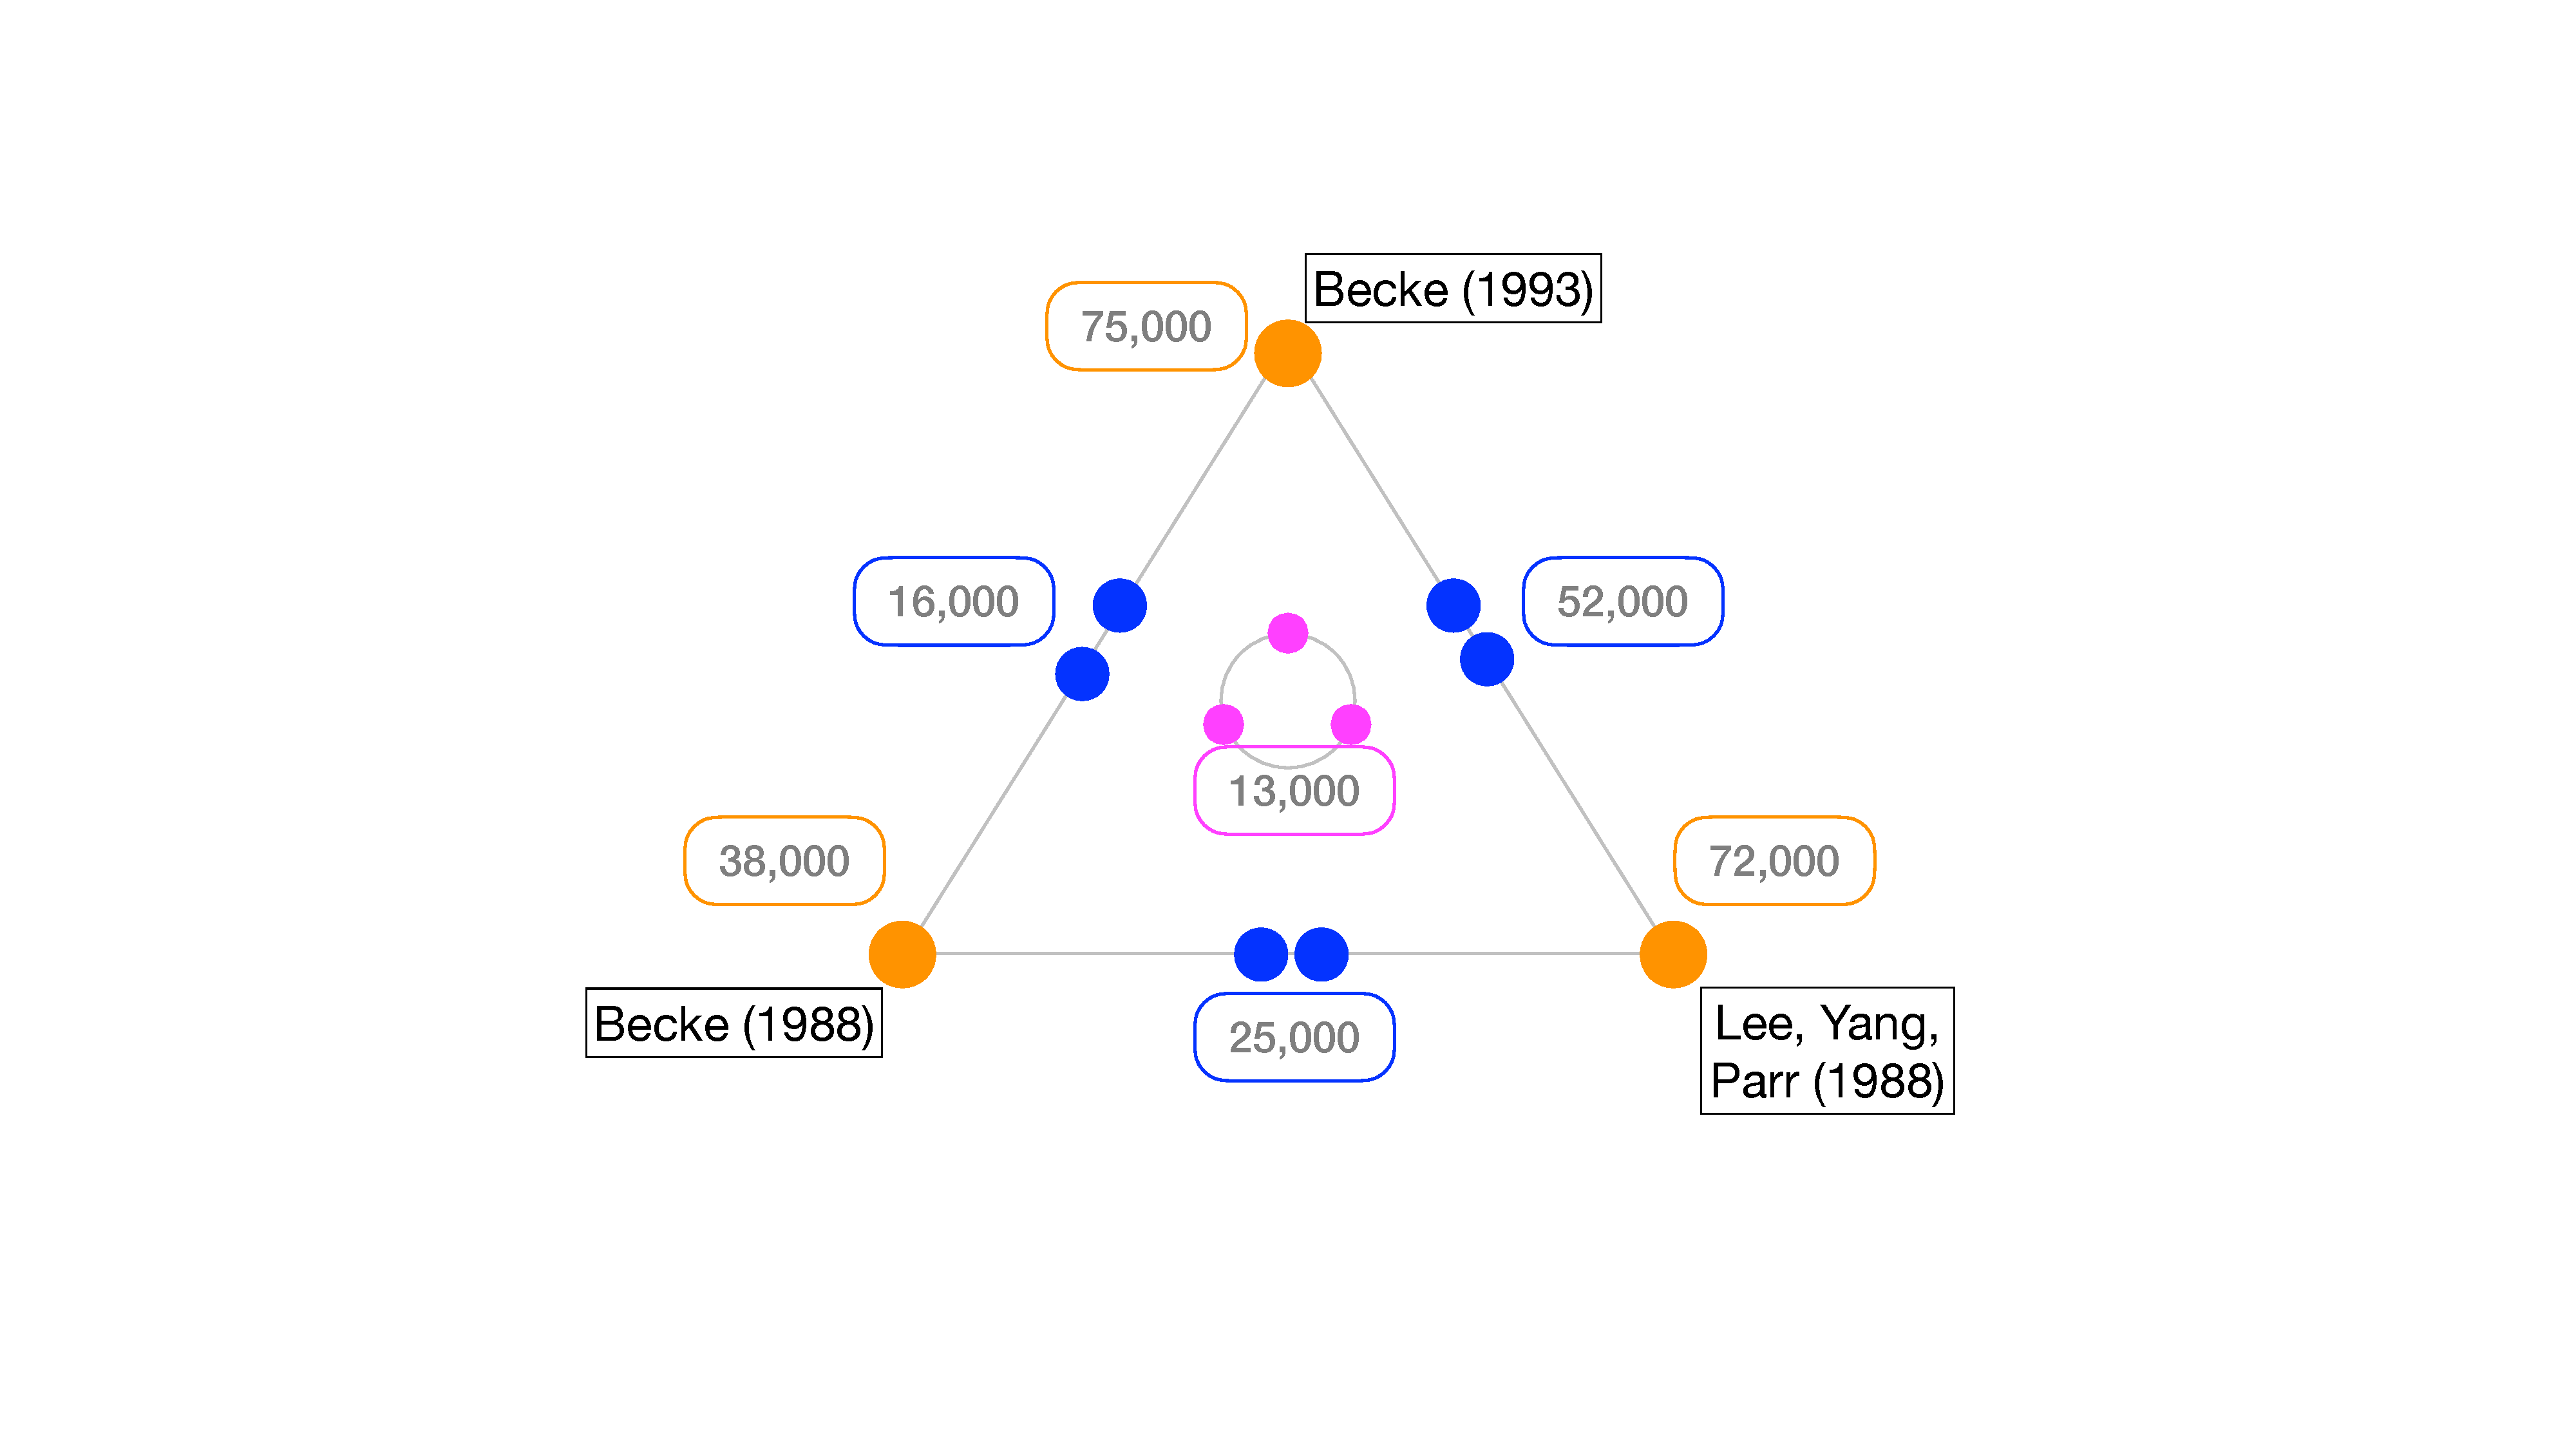
\includegraphics[width=10cm]{fig1_tricite.pdf}% This is a *.eps file
\end{center}
\caption{A high frequency triplet. The triad of (i) Becke (1988), (ii) Becke (1993), and (iii) Lee, Yang, and Parr (1988).  Frequencies (rounded rectangles) are shown for the tri-citation (center of triangle), co-citations (sides of triangle), and 
article citations (vertices of triangle). All frequencies shown have been rounded down to the nearest thousand
}
\label{fig:fig1}
\end{figure}

The first referencing of this triad appears to be in two reports in 1993: (1) an article by Laming, Temath, and Handy titled `A general purpose exchange‐correlation energy functional' and (ii) a chapter titled `Theoretical Organic Chemistry' by Reynolds.  [need to add references]

In 1994, Stephens, Chabalowski, Devlin, and Frisch~\citep{stephens1994ab} blended the Exchange and Correlation functionals into a hybrid functional method referred to as B3LYP (Becke 3-Parameter Lee-Yang-Parr). Historically, B3LYP originates from an effort in the 1980s to to build Exchange and Correlation functionals to allow for the practical application of DFT to chemical problems. A number of research groups engaged and the Becke group in 1988 and 1993 described a hybrid functional~\citep{becke1988density}, and an Exchange functional~\citep{becke1993dft}, respectively, while Lee, Yang, and Parr (LYP) developed a Correlation functional in their 1988 paper~\citep{lyp1988}.  In the B3LYP model, two functionals of the electron density are needed. One is the Exchange functional (two electrons of the same spin cannot be at the same point in space) and the other is the Correlation functional (accounting for the correlated motion of electrons with the same spin). The B3LYP method had a lot of advantages in terms of speed and accuracy, especially for the study of organic molecules, and was rapidly adopted by the computational chemistry and organic chemistry communities.

This major advance can be concisely referenced by citing Becke-1988~\citep{becke1988density}, LYP-1988~\citep{lyp1988} and Becke-1993~\citep{becke1993dft} since the two Becke articles represent the Exchange functional and the Lee-Yang-Parr article contributes the Correlation functional. The high frequency of co-citation (52,000) of Becke-1993 and LYP-1988 may result from authors assuming or concluding that citing Becke's 1993 article is adequate to reference the Exchange functional. 

The three articles in the Becke-1988--LYP-1988--Becke-1993 triad have been co-cited 16,000, 25,000, and 52,000 times respectively, and the individual articles have been cited 38,000, 72,000, and 75,000 times (Figure 1). It is more difficult to conjecture why these three articles are individually cited at these very high levels although it is worth noting that  frequencies of article citations always exceed those of co-citations, which in turn exceed those of tri-citations. It is also very likely that these articles individually stimulated new ideas.

An interesting community discussion thread~\citep{johansson2002} provides the opinion that a complete set of citations for B3LYP is (i) Vosko, Wilk and Nusair, 1980~\citep{vosko1980accurate} or VWN-1980 (ii) Becke-1988) (iii) LYP-1988) (iv) Becke-1993) and (v) Stephens, Chabalowski, Devlin, and Frisch (1994) or SCDF-1994. It is interesting to note that  cite VWN-1980, is not cited in Becke (1988), Becke (1993), or LYP (1993). 

Thus, this high frequency triad discovered through discipline-agnostic citation studies leads us to a cluster of publications that are associated with a major advance in applying DFT to practical use (Kennie needs to approve or rewrite my hand waving). Examining the three component co-cited pairs of the triad allows us to infer that Becke (1993) and LYP (1988) are most extensively recognized in the community as far as B3LYP is concerned. 

%\bibliographystyle{acm}
\bibliography{B3LYP}



\end{document}  